\documentclass[handout,noauthor,nooutcomes]{ximera}

\input{../../../../preamble.tex}

\usepackage{multicol}

\title[Collaborate:]{Identifying surfaces}

\begin{document}
\begin{abstract}
We identify surfaces.
\end{abstract}
\maketitle

\textbf{Work in groups of 3--4, writing your answers on a separate
  sheet of paper.}

Match the following functions to the level curves. %% COPIED FROM SCHENK
\begin{multicols}{2}
\begin{enumerate}
\item $3xy-x^3-y^3+\frac{1}{16}$
\item $\frac{3x}{2} -\frac{x^3}{2} - xy^2+\frac{1}{16}$
\item $x^4-2x^2+y^2-\frac{17}{16}$
\item $-2x^3-3y^4+6xy^2+\frac{1}{16}$
\item $x^4-y^4-2x^2+2y^2+\frac{1}{16}$
\item $-x^4+4xy-2y^2+ \frac{1}{16}$
\end{enumerate}
\end{multicols}

\begin{multicols}{2}
  \renewcommand{\theenumi}{(\roman{enumi})}
  \begin{enumerate}
  \item \raisebox{-.5\height}{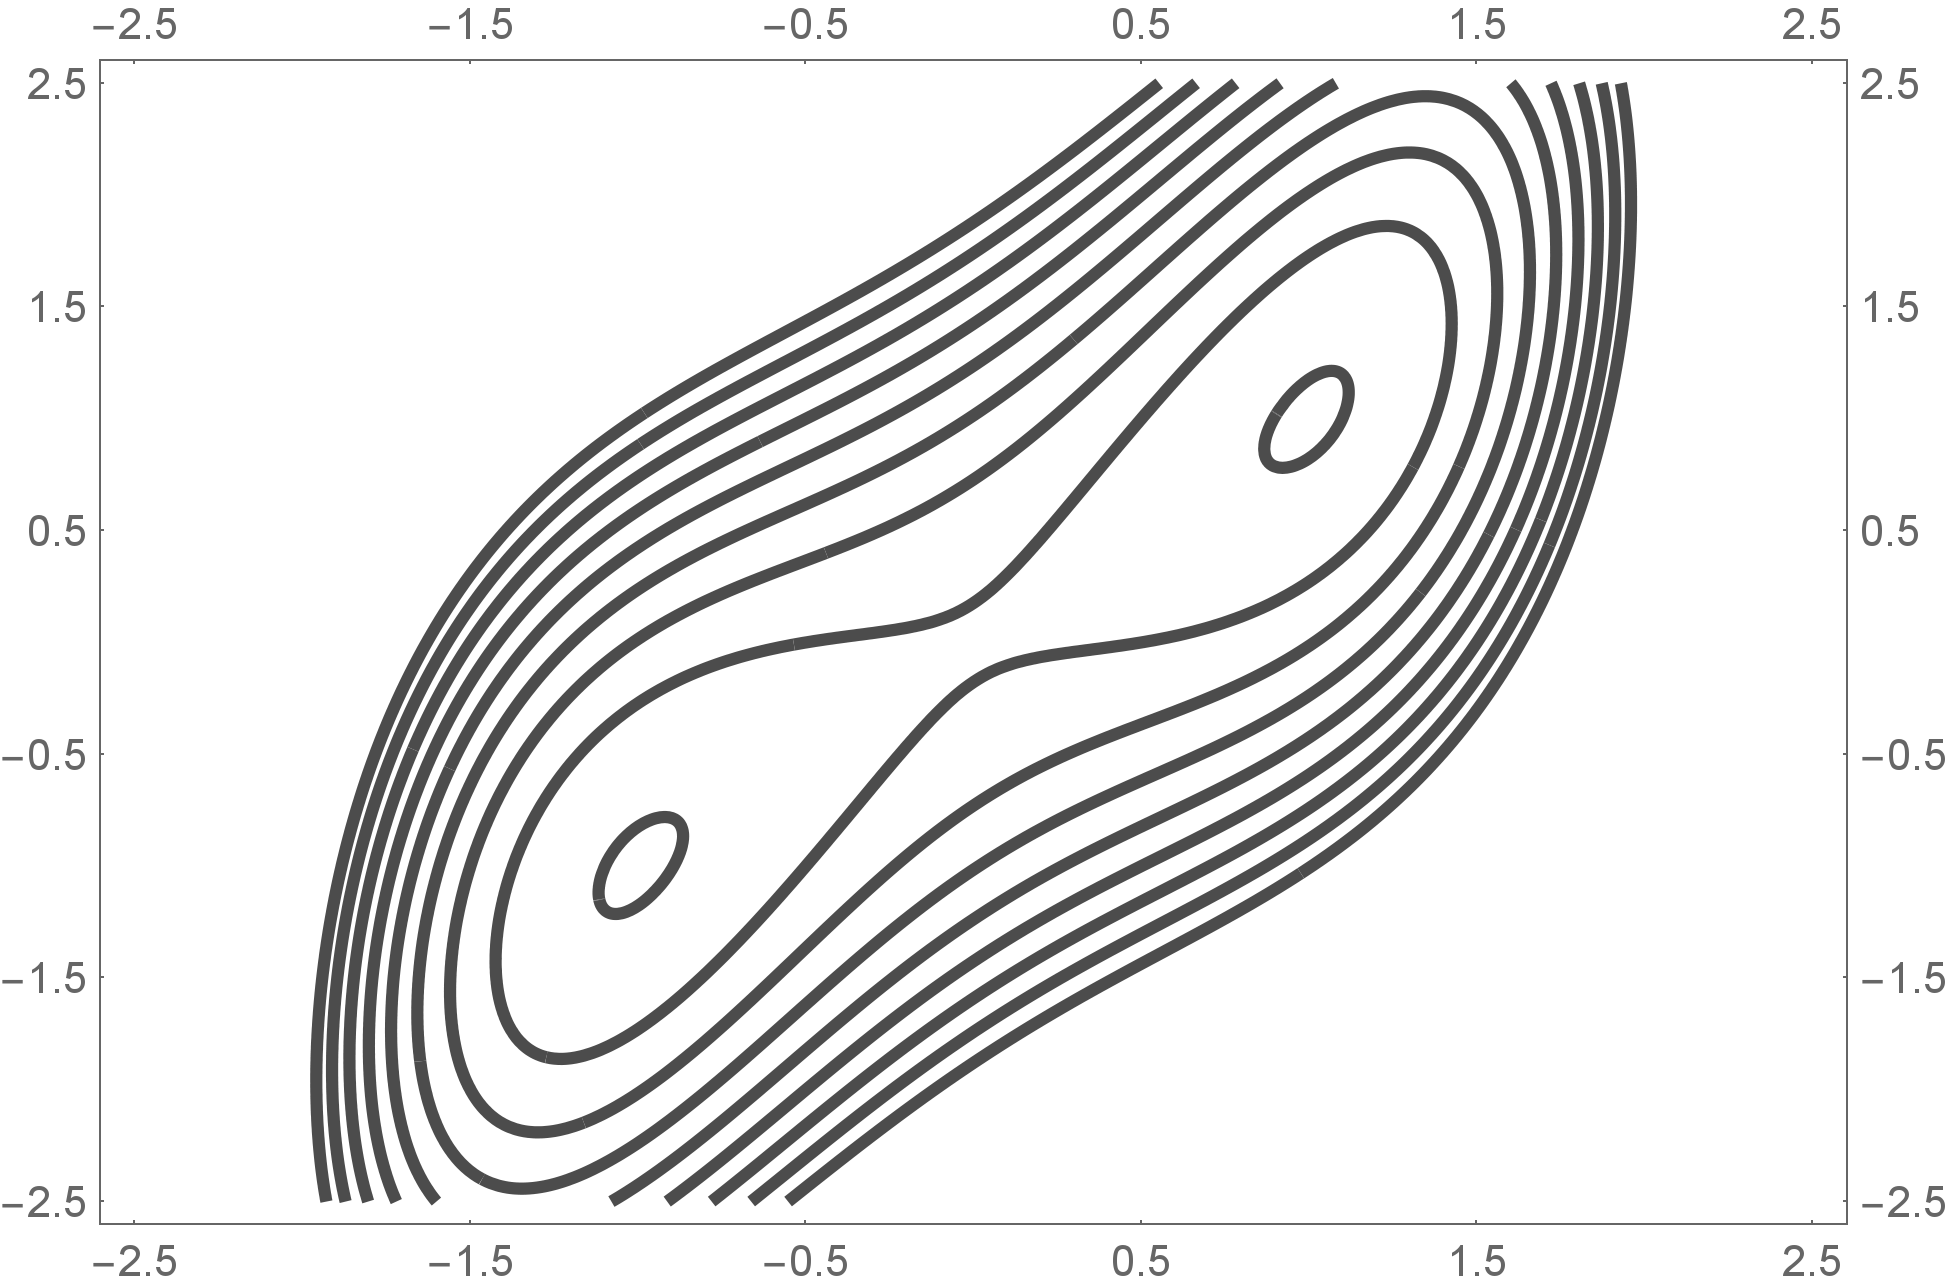
\includegraphics[width=2in]{surfaceF}}
  \item \raisebox{-.5\height}{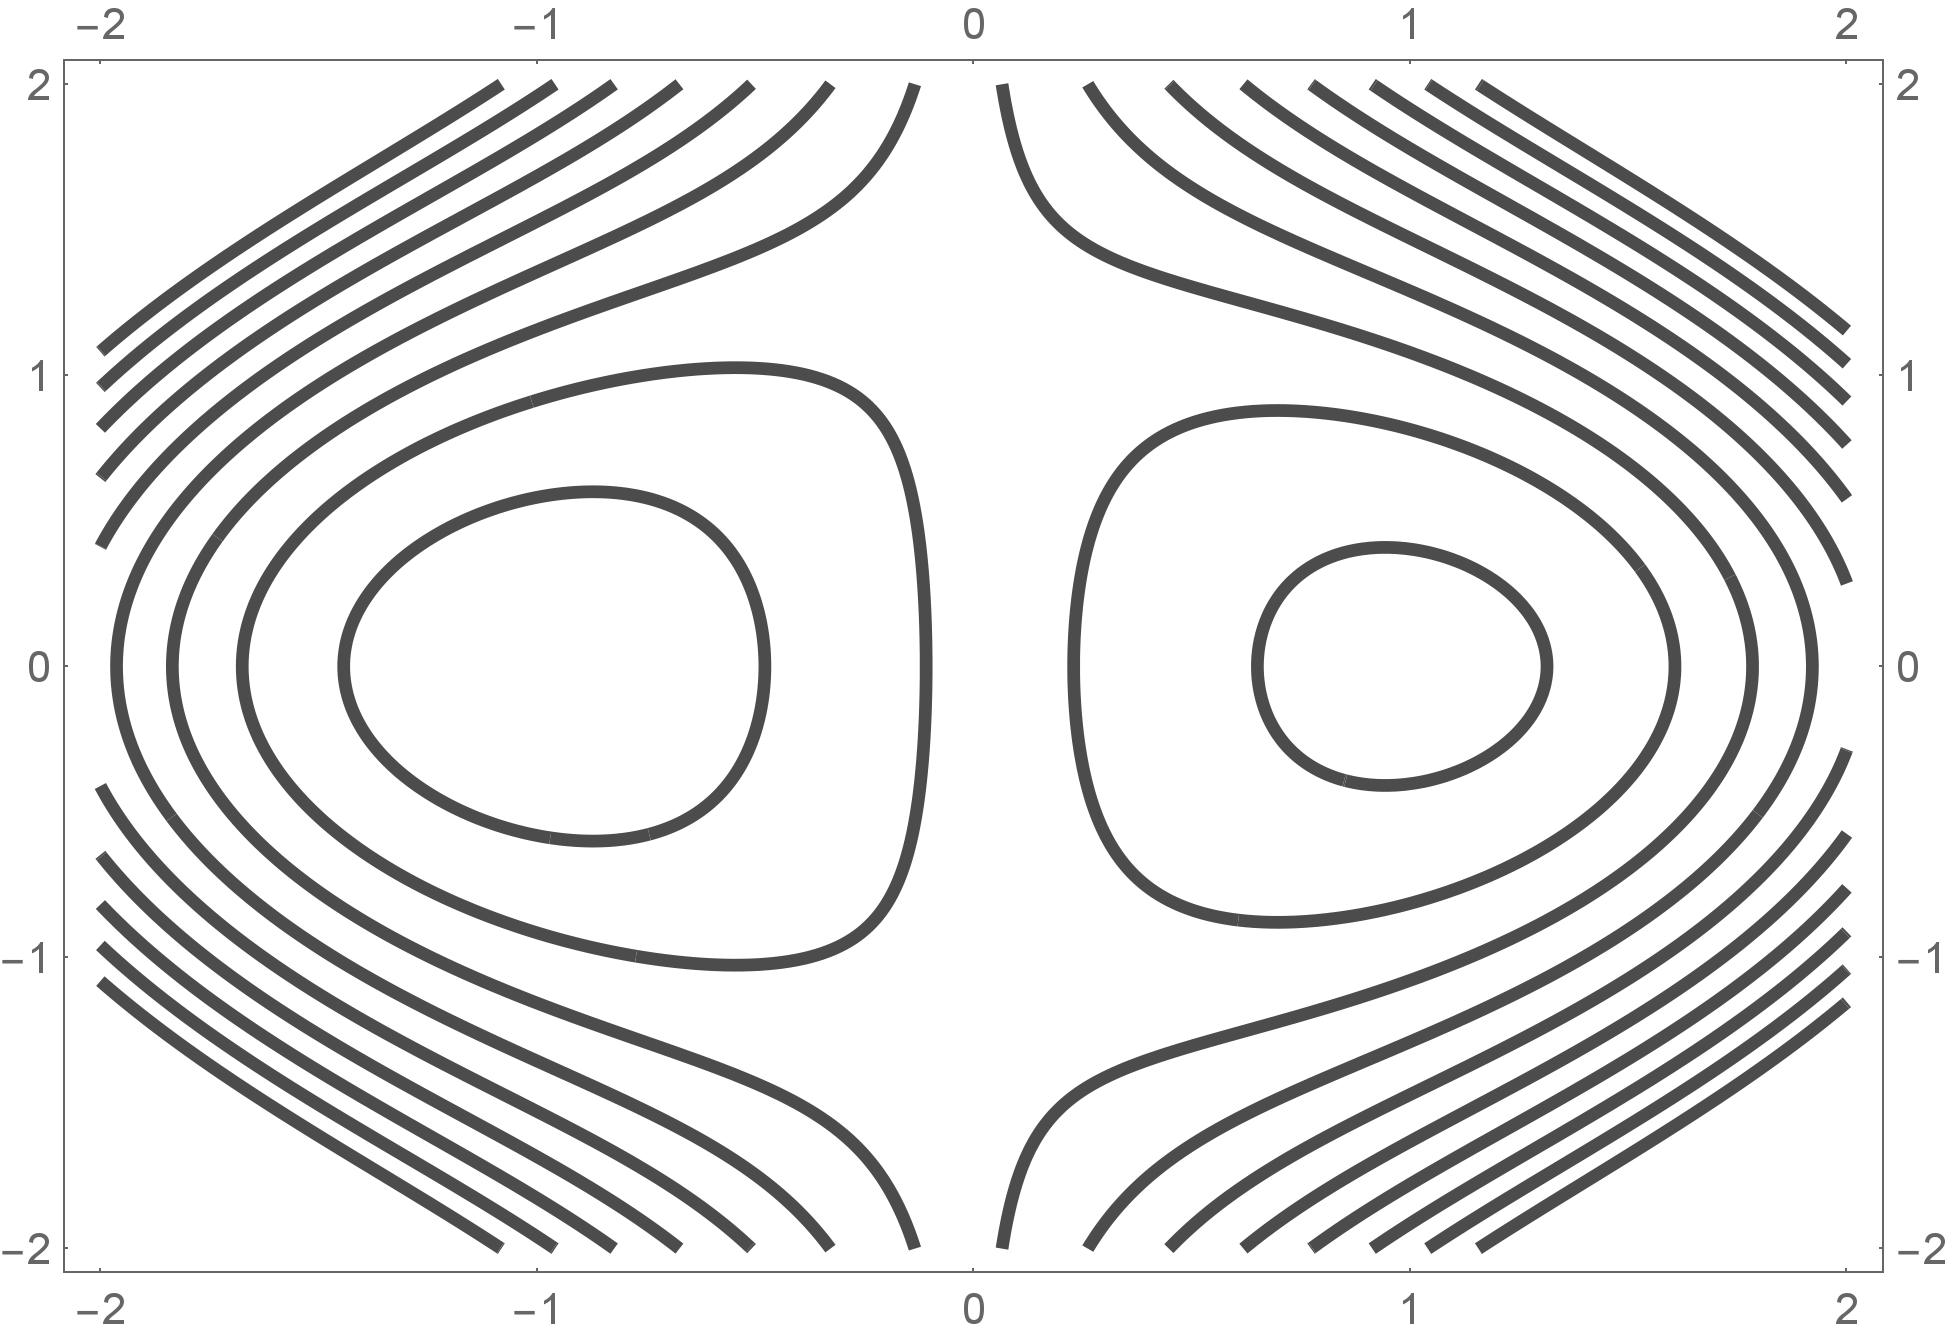
\includegraphics[width=2in]{surfaceB}}
  \item \raisebox{-.5\height}{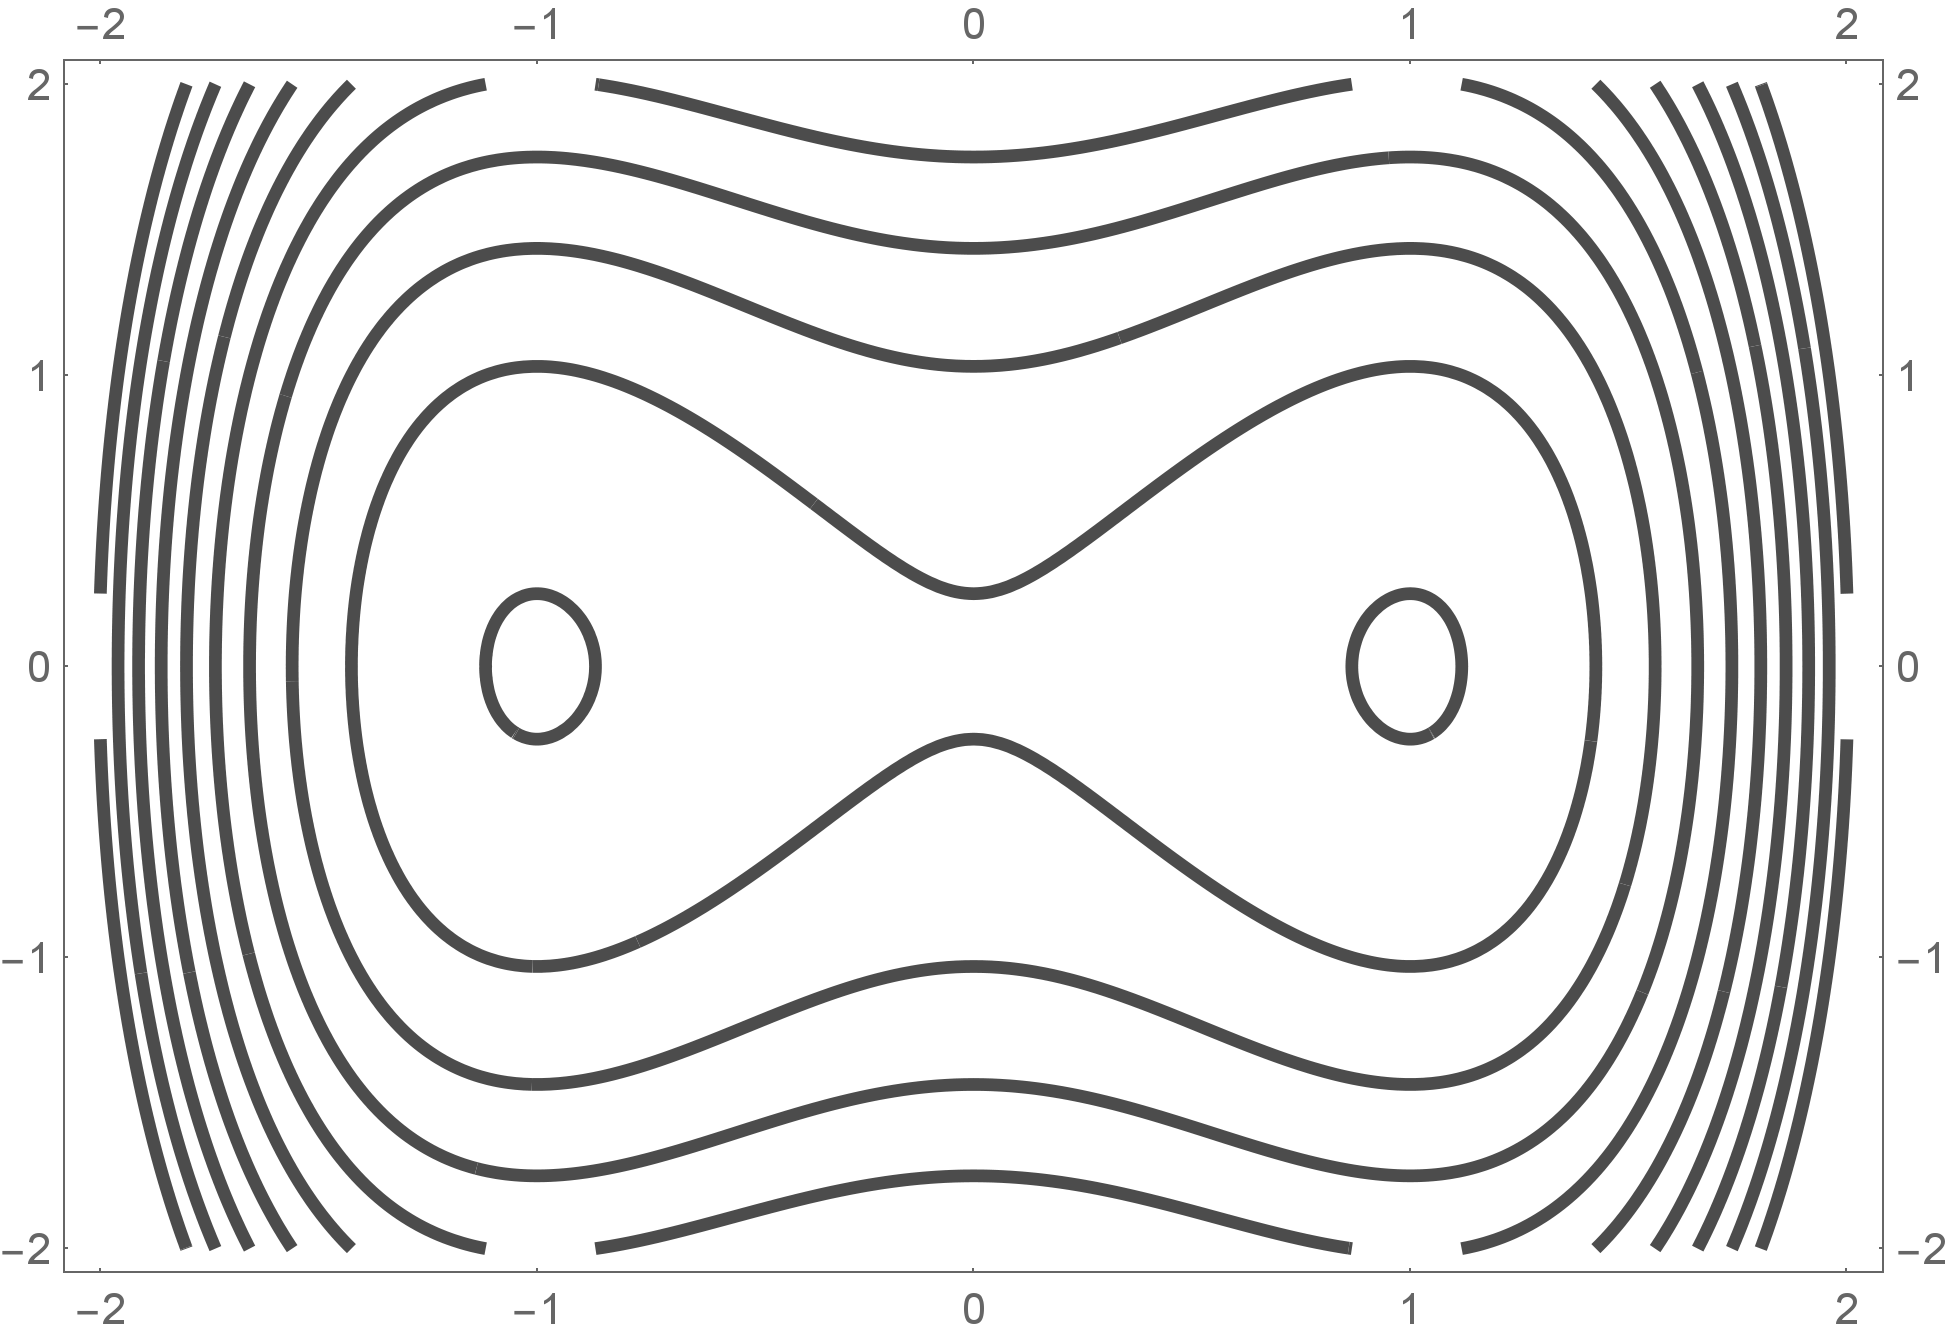
\includegraphics[width=2in]{surfaceC}}
  \item \raisebox{-.5\height}{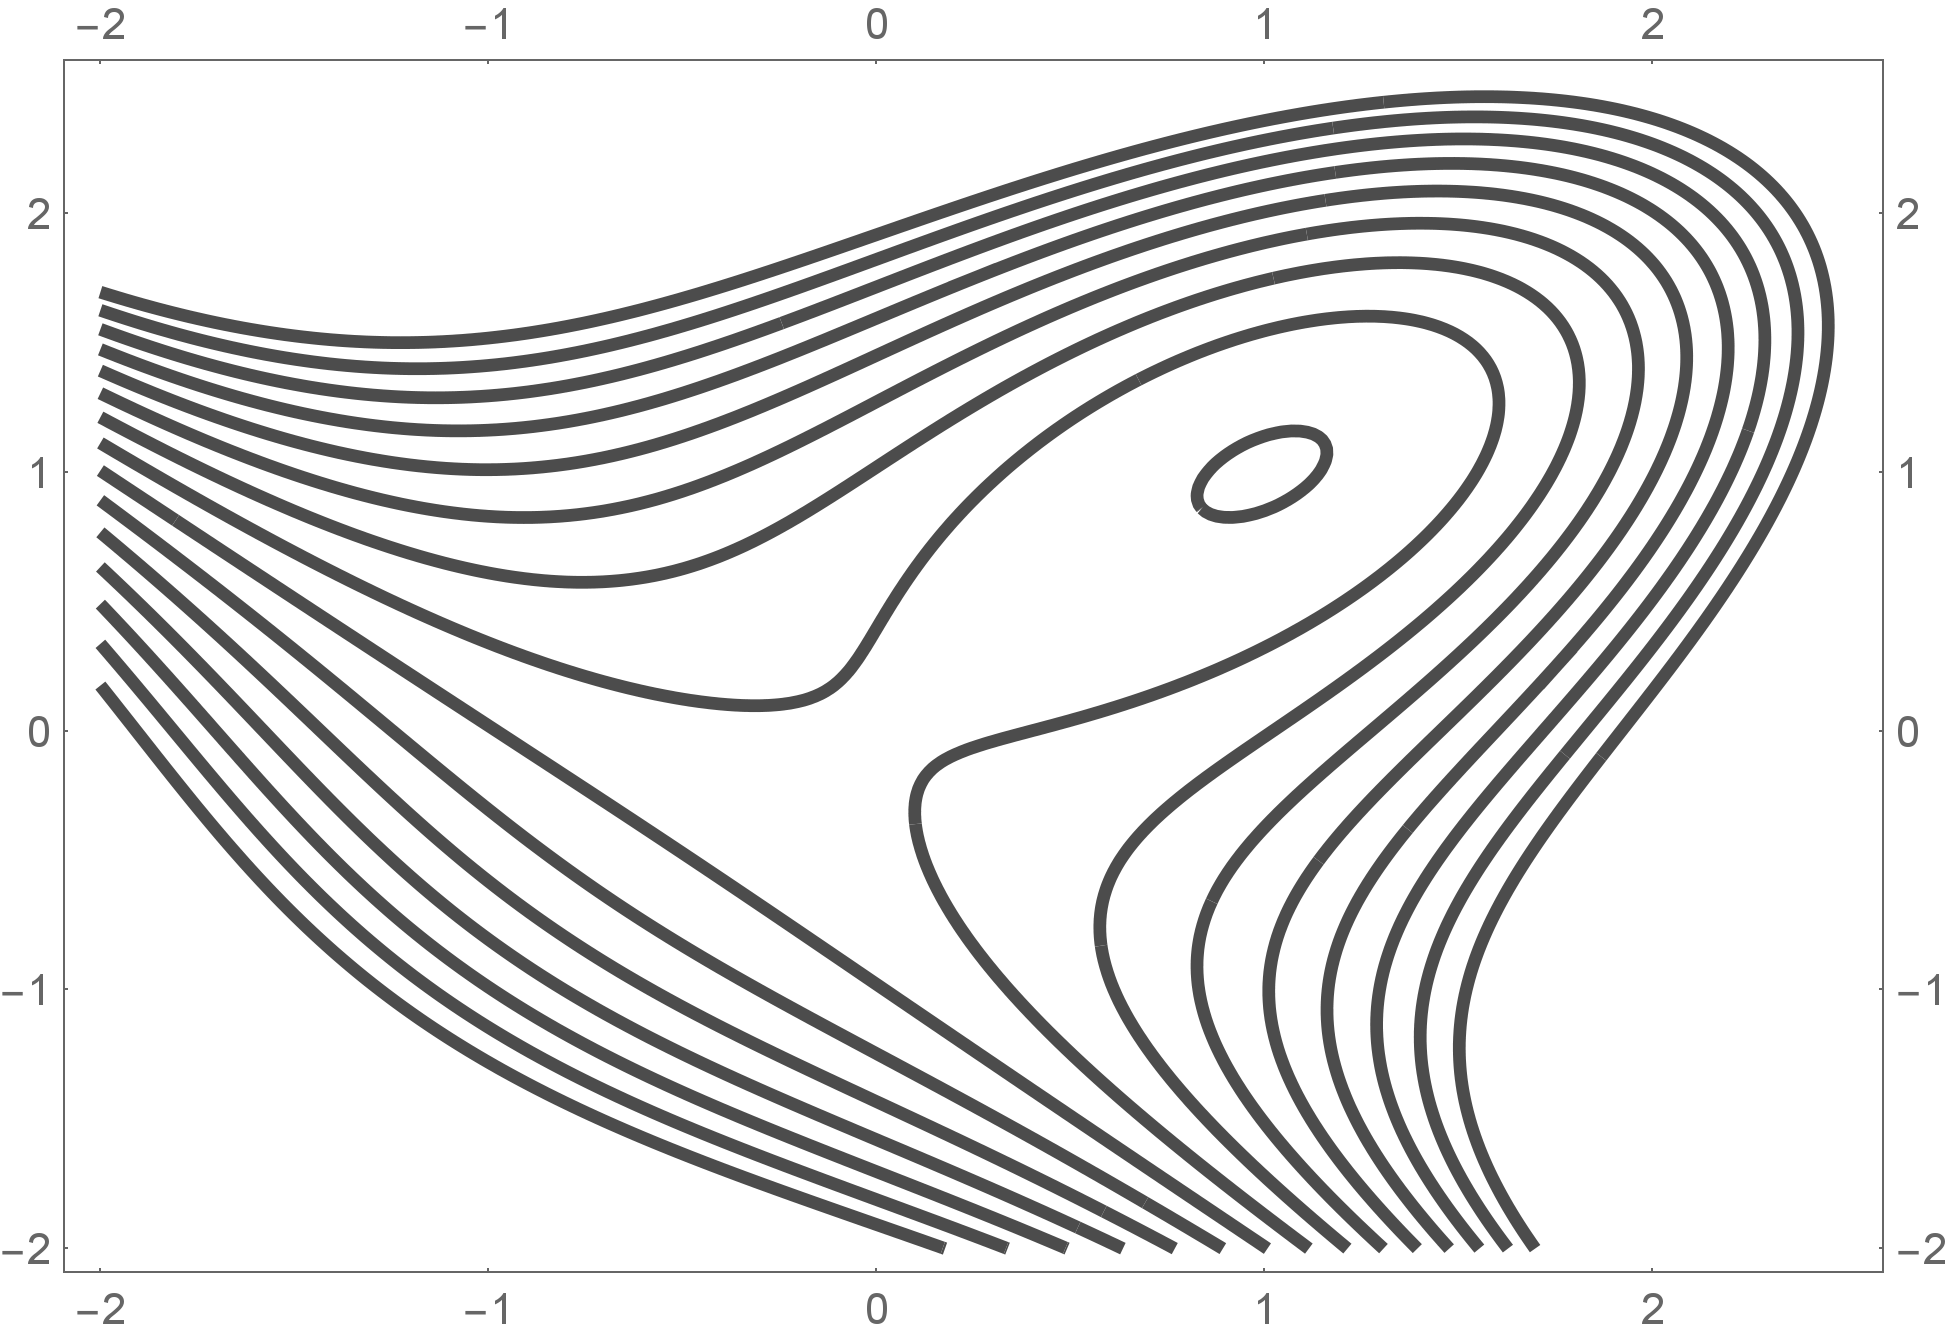
\includegraphics[width=2in]{surfaceA}}
  \item \raisebox{-.5\height}{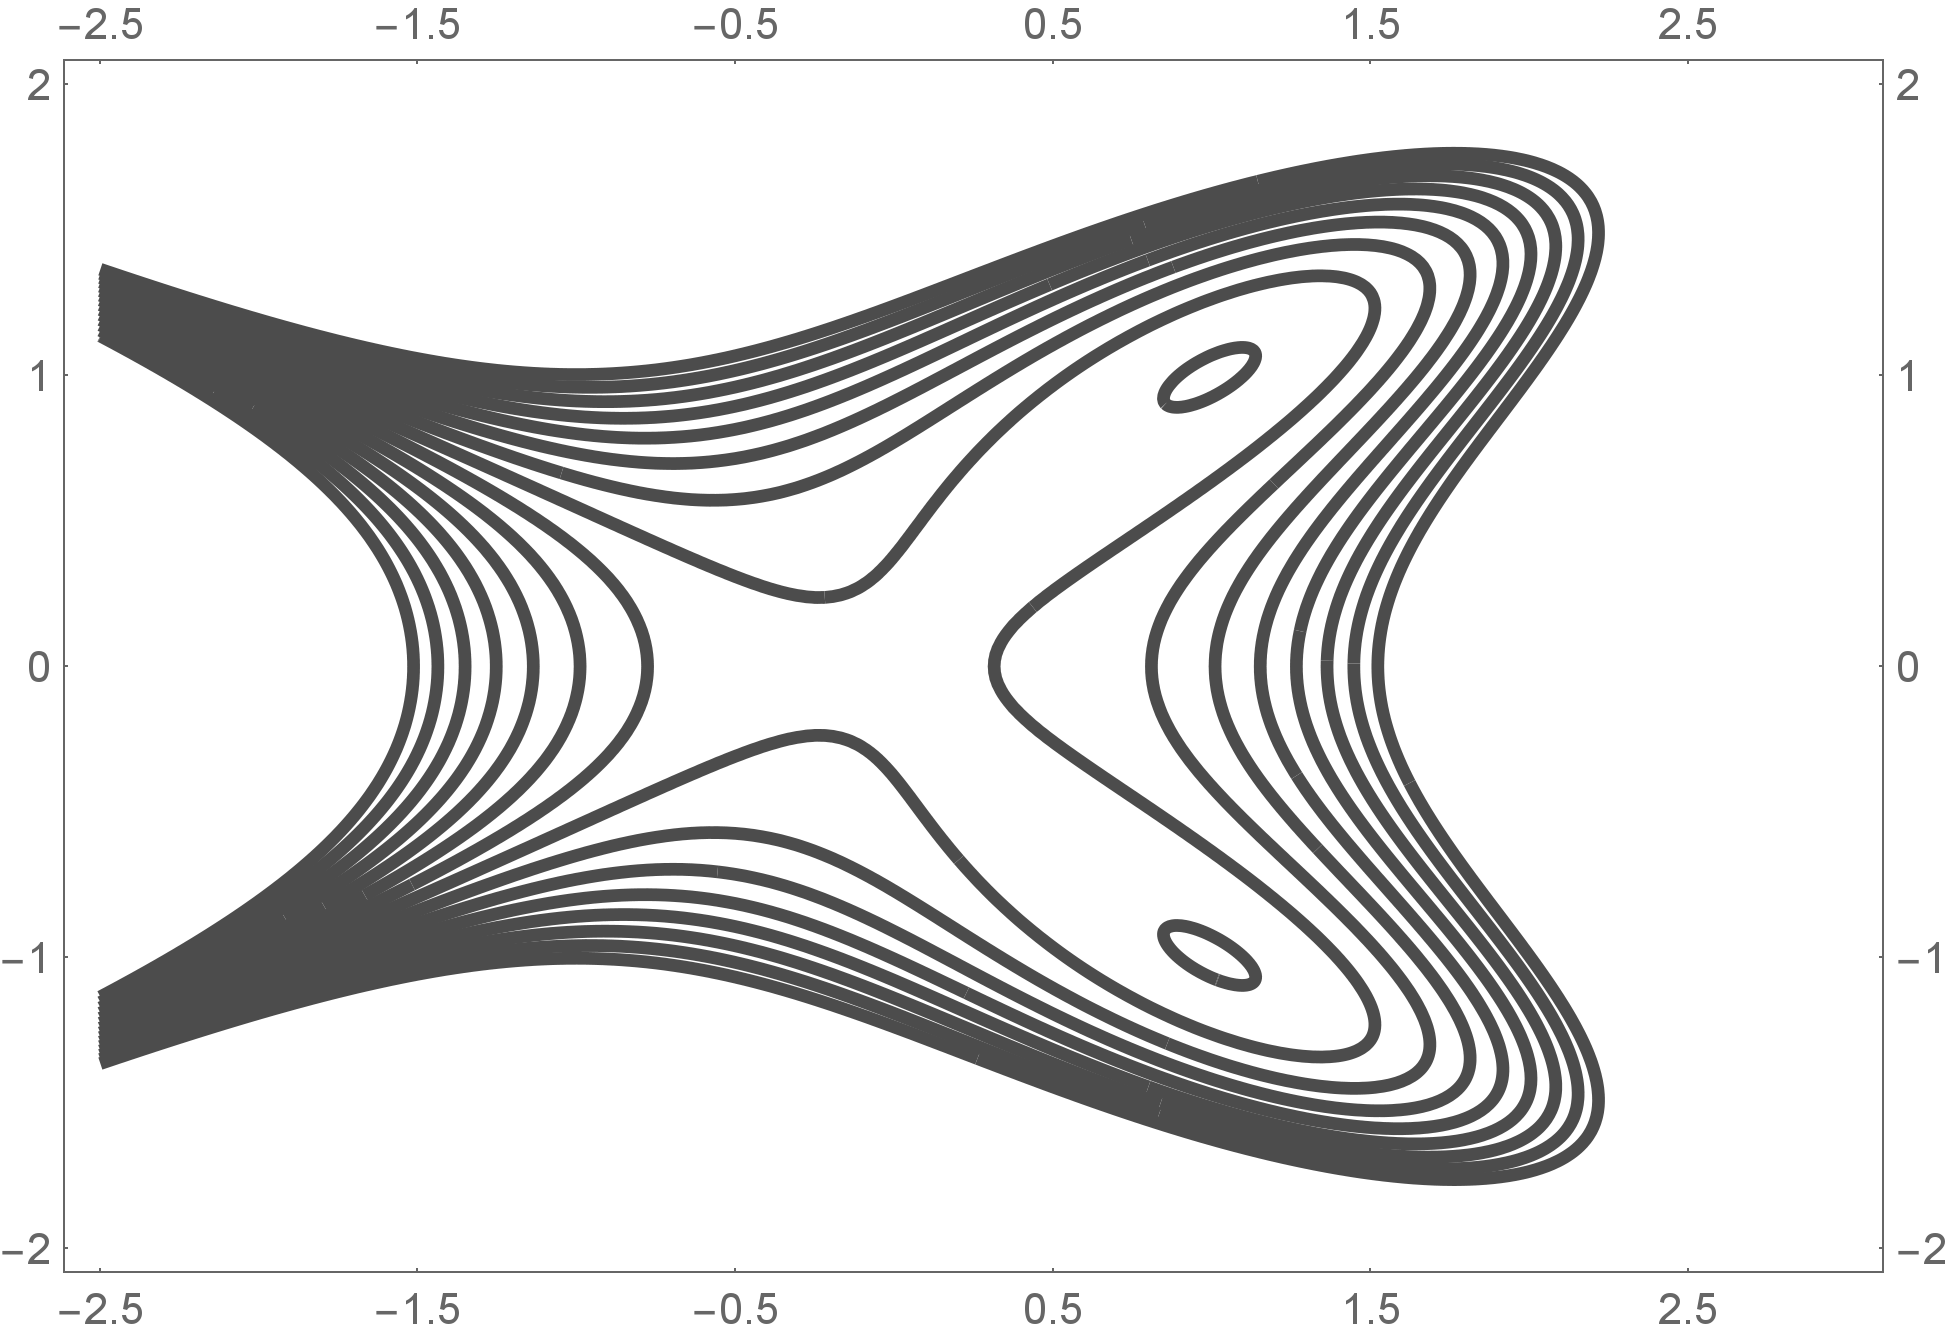
\includegraphics[width=2in]{surfaceD}}
  \item \raisebox{-.5\height}{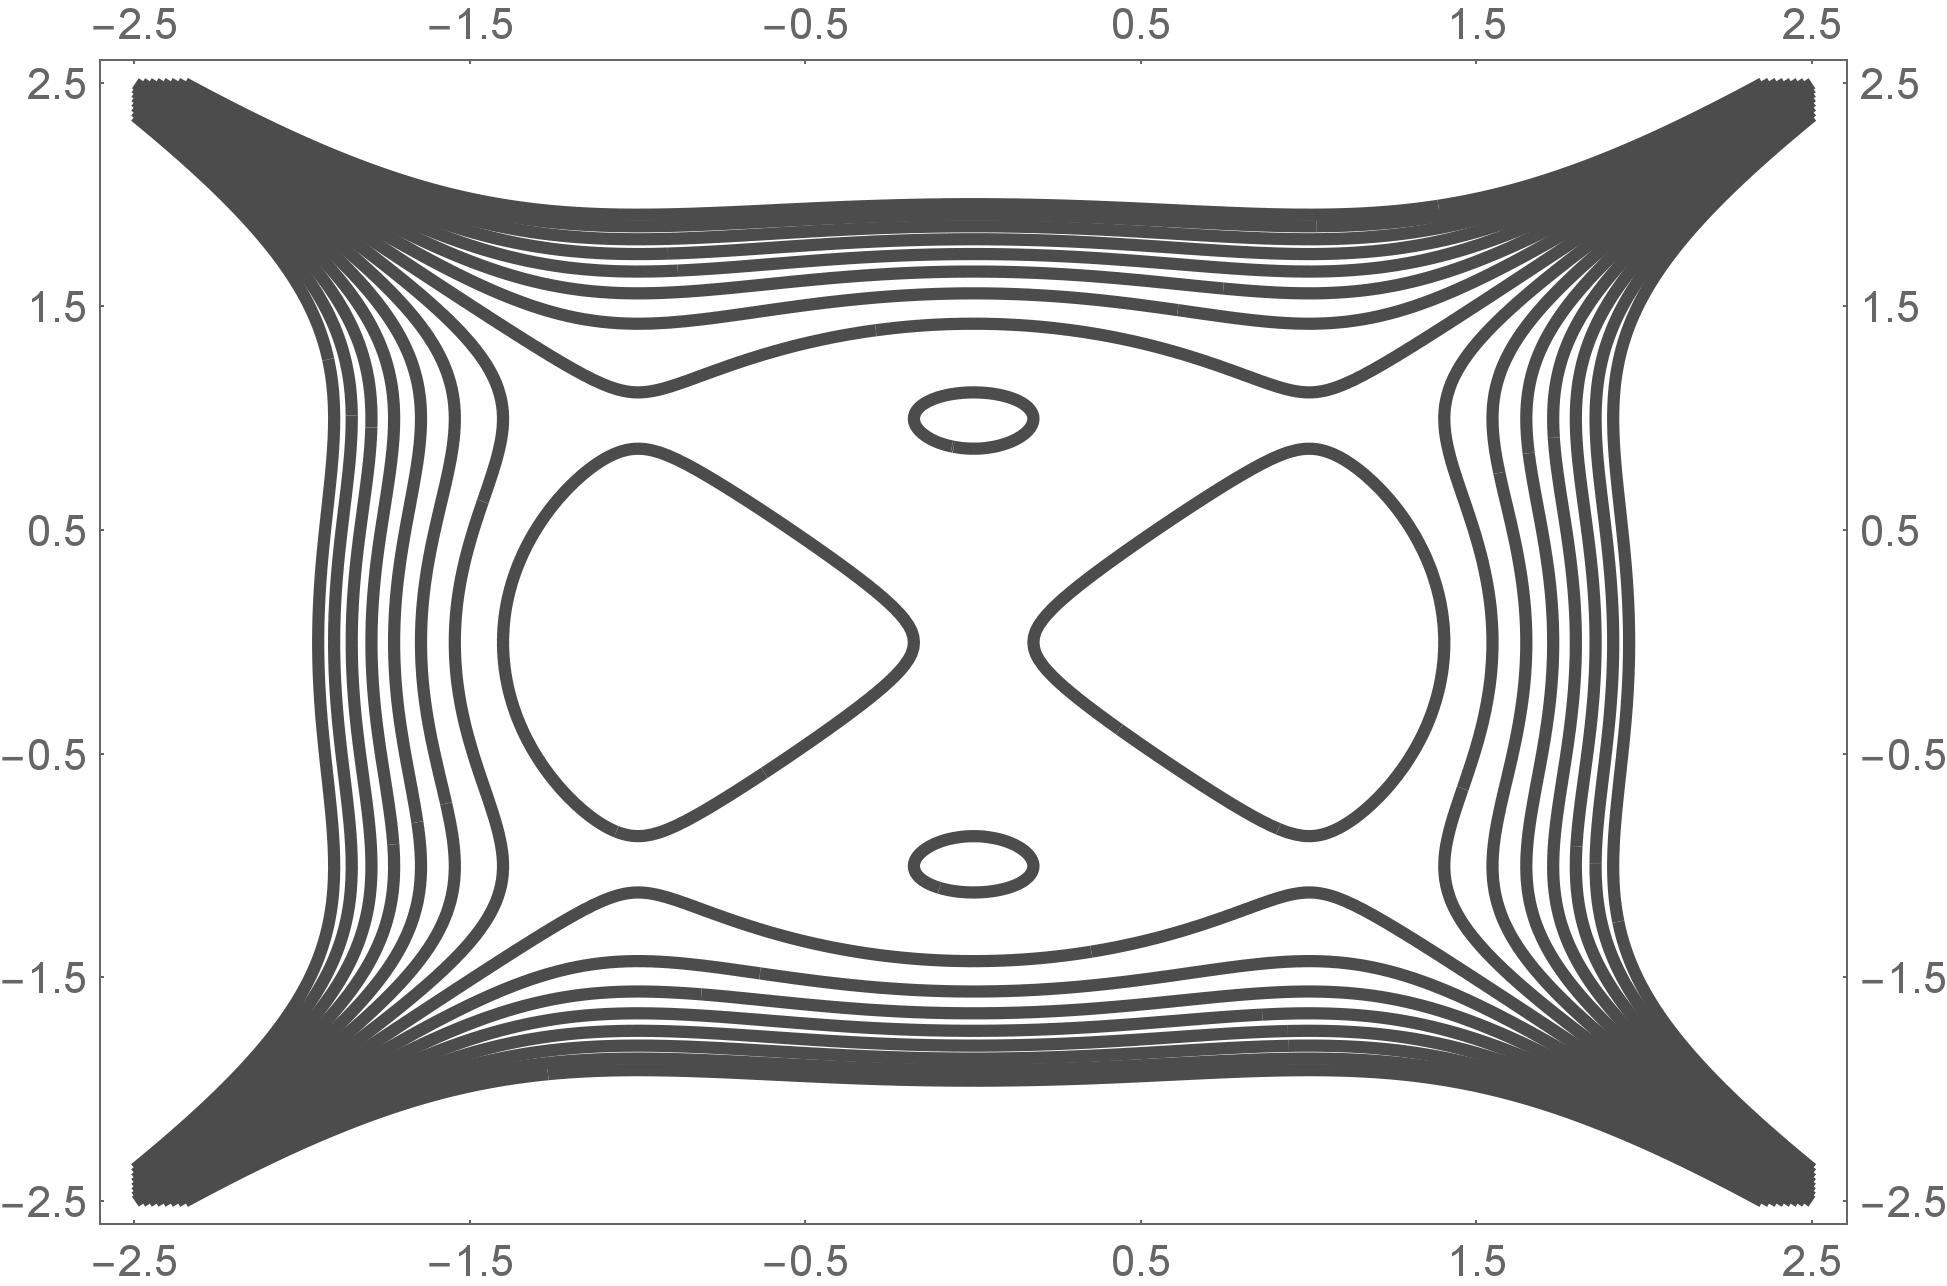
\includegraphics[width=2in]{surfaceE}}
  \end{enumerate}
\end{multicols}
\end{document}
